\toclesssection{SCP 030 - The Homunculus}
\addcontentsline{toc}{section}{SCP 030 - The Homunculus}

\textbf{Item \#:} SCP-030

\textbf{Object Class:} Safe

\begin{figure}[h]
\begin{center}
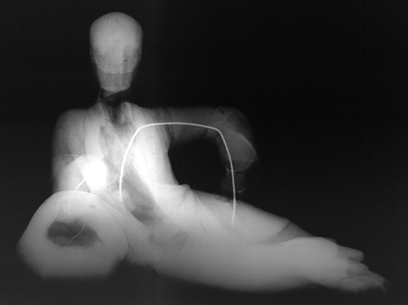
\includegraphics[scale=0.55]{scp/030.jpg}
\linebreak An X-Ray image of SCP-030. The solid white line running from the core through the left arm is a portion of its tracking system.
\end{center}
\end{figure}

\textbf{Special Containment Procedures:} SCP-030 is confined to Site 62 with a special security grade (Class F) allowing it access to all unsecured research labs, records facilities and communal social areas (mess halls, dormitories, gymnasiums) when accompanied by at least one (1) staff member Class 1 or higher. With the written consent of Level 4 personnel, SCP-030 may be granted temporary access to secured research labs or Euclid-class SCP containment facilities to act as a research assistant under the direct supervision of assigned laboratory staff.

SCP-030 has been equipped with a tracking device so its location within Site 62 can be determined precisely at any time. Tracking software is installed on all computers for Class 3 staff and higher.

\textbf{Discovery:} SCP-030 was discovered 6/12/\censor{XXXX} on the grounds of the cemetery of \censor{XX} \censor{XXXX} \censor{XXXXXXXXX}'s Church in London's Mortlake District. It was buried in an unmarked plot approximately 2.7 meters (9 feet) in depth, contained in a small stone sarcophagus. The sarcophagus bore no markings and was assumed to be that of a deceased infant. The sarcophagus lid was shattered by a careless local historian during the excavation, exposing SCP-030 to daylight. Upon being struck by the sun's rays, SCP-030 roused from its inert state to one of mild activity within a few seconds, stating simply, "Good afternoon." A member of the Foundation's Greater London recon force was summoned within hours and took the specimen into custody without resistance.

\textbf{Description:} SCP-030 appears as a hairless, genderless, grey-toned human approximately 71 centimeters (28 inches) in height. Its solid blue eyes lack discernible irises or pupils, rather resembling two small cut sapphires. SCP-030 possesses a vaguely masculine voice with a pronounced English accent and is able to converse, read and write in Ancient Greek, Latin, Italian, English, Spanish and Portuguese as well as two (2) additional languages that have not yet been identified despite SCP-030's insistence that they should be "common knowledge." SCP-030 offers regular lectures on these languages to Site 62 staff. SCP-030 has also demonstrated knowledge of physics, chemistry, astronomy, mathematics and horticulture at roughly a postgraduate level.

SCP-030 remains active while a source of light equivalent to a candle flame is within 1.5 meters (5 feet). In the absence of light, SCP-030 becomes inert, apparently losing consciousness and showing no outward signs of life. Within five to ten (5-10) seconds of being re-exposed to light, SCP-030 becomes active once more, appearing to come out of a light slumber no matter how long the period of inactivity has been. SCP-030 does not appear to require these periods of inactivity as a human would require sleep, preferring to remain active so long as there is a human nearby that it can be of use to.

Biopsy analysis of SCP-030 remains inconclusive. While clays native to English soil seem to make up the majority of its structure, traces of mandrake (Mandragora officinarum), lye, mercury, and human blood have been found in each sample taken. SCP-030 has expressed that a full exploratory surgery to determine its workings would no doubt end its existence and provide no further answers. Due to its utility in research, no plans have been made to examine SCP-030 beyond regular monthly physicals.

SCP-030 appears to require no sustenance and produces no waste, although it does occasionally request a bath. When questioned regarding its origins, it replies that it has been "asked to forget that bit of information", but offers able assistance and insight into any current problem to which it is applied. It has denied any prior knowledge of other SCP's contained on-site and has politely refused to enter any SCP containment enclosure without ample human security accompaniment. To date, SCP-030 has been responsible for no less than 6000 hours of research assistance to Site 62 staff across multiple departments and command levels. Despite the opportunity, SCP-030 has shown no desire to escape the confines of Site 62, regularly reporting that it "has plenty to help with around here, thank you."
\newpage
\textbf{Document 030-C:} Security logs for SCP-030

9/14/\censor{XXXX}: The entity designated SCP-030 ("Ariel") is granted provisional Security Access Level F, to be revoked at any time by administrative staff Class 4 or higher. Tracking system installed.

12/21/\censor{XXXX}: SCP-030 reports malfunction of its own tracking system. Repairs completed within six (6) hours. SCP-030 offers to assist, but is refused for security purposes.

3/13/\censor{XXXX}: SCP-030 completes 18-week seminar on Unknown Language Alpha ("Zephyr"), five (5) staff researchers considered fluent. Lexicography transmitted to O5-\censor{X}.

6/16/\censor{XXXX}: SCP-030 has requested materials and lab space for independent research. Approval pending.